\chapter{Συμπεράσματα - Μελλοντική Έρευνα}

Παρακάτω συνοψίζουμε τις μεθόδους που αναλύσαμε κατά τη διάρκεια της εργασίας αυτής και εξάγουμε συμπεράσματα. Στη συνέχεια αναφέρουμε επεκτάσεις, μελλοντικά έργα και νέα μοντέλα προστασίας που παρουσιάστηκαν πρόσφατα. Τέλος παρουσιάζουμε ορισμένα ανοικτά ζητήματα πάνω στην προστασία της ιδιωτικότητας των δεδομένων που θα μας απασχολήσουν στο άμεσο μέλλον.

\section{Σύνοψη και συμπεράσματα}

Στην εργασία αυτή ασχοληθήκαμε με την μελέτη των μεθόδων προστασίας της ιδιωτικότητας των δεδομένων. Μιλήσαμε για την επικινδυνότητα αποκάλυψης πληροφορίας που προκύπτει από την εφαρμογή απλών τεχνικών ανωνυμοποίησης, και την ανάγκη εισαγωγής πολυπλοκότερων μεθόδων. Αναλύσαμε τις κυριότερες τεχνικές γενίκευσης, τονίζοντας τόσο τα πλεονεκτήματα, αλλά και τα μειονεκτήματα της κάθε μιας. Παρουσιάσαμε την επίθεση τομής η οποία διαπερνά, θεωριτικά, κάθε μέθοδο γενίκευσης. Στη συνέχεια αναλύσαμε σε βάθος την μέθοδο της διαφορικής ιδιωτικότητας και τους μηχανισμούς τυχαιοποίησης που την συνοδεύουν. Τέλος, αναπτύξαμε κώδικα σε γλώσσα προγραμματισμού \textlatin{Python} που εφαρμόζει τον μηχανισμό \textlatin{Laplace} και εκτελέσαμε παραδείγματα τυχαιοποίησης σε ένα σύνολο δεδομένων.




Όπως είδαμε, ένα σύνολο δεδομένων στο οποίο έχουν εφαρμοστεί μηχανισμοί ανωνυμοποίησης μπορεί να εξακολουθεί να παρουσιάζει κινδύνους αποκάλυψης για τις εγγραφές στις οποίες αναφέρονται τα δεδομένα. Ακόμα και σε περίπτωση μη ανάκτισης της ταυτότητας ενός ατόμου, ενδέχεται να είναι εφικτή η αποκάλυψη στοιχείων σχετικά με το συγκεκριμένο άτομο με τη βοήθεια συνήθως άλλων πηγών πληροφοριών. Οφείλουμε λοιπόν να υπογραμίσουμε ότι καμία από τις τεχνικές που περιγράφονται στην παρούσα εργασία δεν πληροί με βεβαιότητα τα τρία κριτήρια της αποτελεσματικής ανωνυμοποίησης\footnote{Παράγραφος \ref{kri}}. Ωστόσο, ορισμένοι απο τους κινδύνους αυτούς ενδέχεται να μπορούν να αντιμετοπιστούν εξ' ολοκλήρου από μια συγκεκριμένη μέθοδο, δεδομένου ότι έχουν γίνει οι απαραίτητοι χειρισμοί κατα την ανάπτυξη της. Ο παρακάτω πίνακας απεικονίζει τις δυνατότητες των μηχανισμών ανωνυμοποίησης που αναλύσαμε.

\begin{figure} [h!]
\begin{center}
  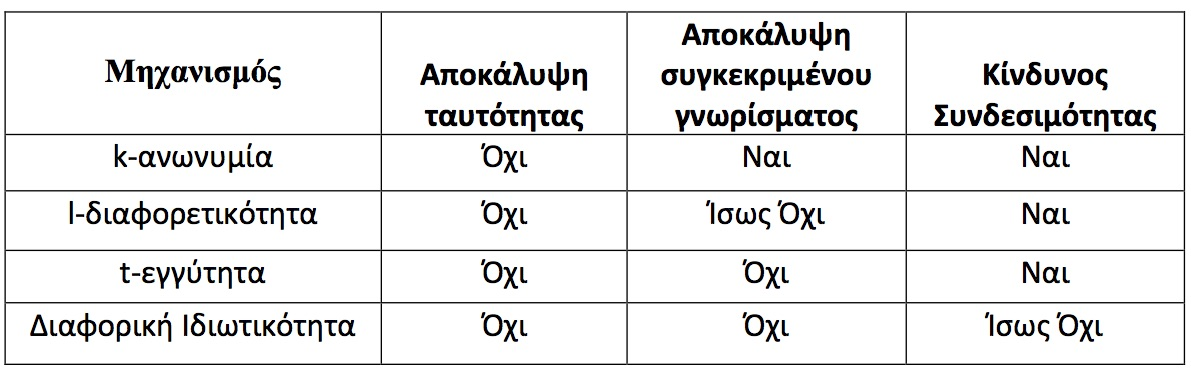
\includegraphics[scale=0.31]{images/mhx.jpg}
  \caption{Πλεονεκτήματα και μειονεκτήματα τεχνικών ανωνυμοποίησης}
  %\label{fig:boat1}
  \end{center}
\end{figure}


Συνεπώς, καλό είναι να εφαρμόζεται ο κάθε μηχανισμός ιδιωτικότητας σε αντίστοιχες περιπτώσεις ανωνυμοποίησης ανάλογα με τις απαιτήσεις του υπεύθυνου της βάσης δεδομένων ή ακόμη καλύτερα, η ταυτόχρονη χρήση διαφορετικών μηχανισμών στο ίδιο σύνολο δεδομένων. 
%Η μέθοδος της διαφορικής ιδιωτικότητας όπως είδαμε βοηθά στην επιλογή κατάλληλου επιπέδου θορύβου ώστε το αποτέλεσμα να ισορροπεί μεταξύ ποιότητας-ιδιωτικότητας. Πέραν της χρήσης του \textlatin{Laplace} και των άλλων βασικών μηχανισμών της μεθόδου, μπορεί ο διαχειριστής να χρησιμοποιήσει πιο σύνθετες εφαρμογές, ανάλογα με τις συνθήκες που αντιμετωπίζει.  






\section {Νέες τεχνικές - συνδυασμοί}

Εχουν προταθεί τον τελευταίο καιρό νέες μέθοδοι ανωνυμοποίησης δεδομένων αλλά και συνδυασμοί τεχνικών γενίκευσης-τυχαιοποίησης οι οποίες υπόσχονται ακόμη καλύτερα αποτελέσματα.

Πιο συγκεκριμένα, οι συνεχείς απαιτήσεις για προστασία των όλο και μεγαλύτερων συνόλων δεδομένων, οδηγούν σε έρευνες οι οποίες επιδιώκουν να συνδυάσουν τις μεθόδους ανωνυμοποίησης που αναφέραμε, με σκοπό ασφαλέστερα και ταχύτερα αποτελέσματα. Ένας συνδιασμός που αξίζει να ανφέρουμε είναι η χρήση τεχνικών γενίκευσης και διαφορικής ιδιωτικότητας \textlatin{\cite{DBLP:journals/corr/Domingo-FerrerS15a}}.
Στην εργασία αυτή αποδεικνύεται ότι η $k$-ανωνυμία για την προστασία των \textlatin{quasi-identifiers}, σε συνδιασμό με μηχανισμό $\epsilon$-διαφορικής ιδιωτικότητας για τα ευαίσθητα γνωρίσματα αποδίδει στοχαστική $t$-εγγύτητα \footnote{επέκταση της $t$-εγγύτητας}, με $t=t(k,\epsilon)$ συνάρτηση των $k$ και $\epsilon$. 


Πέραν αυτού, πρόσφατες έρευνες αναδεικνύουν νέα μοντέλα προστασίας της ιδιωτικότητας των δεδομένων, τόσο διαδραστικά όσο και μη διαδραστικά. 
Τελευταία, παρουσιάστηκε η τεχνική \textlatin{permutation paradigm} για να περιγράψει οποιαδήποτε μέθοδο κάλυψης δεδομένων, κυρίως \textlatin{microdata}, ως «μεταλλαγή», ανοίγοντας το δρόμο για την πραγματοποίηση ουσιαστικών αναλυτικών συγκρίσεων των μεθόδων\textlatin{\cite{domingo2016new}}. 
Η ιδιωτικότητα που εξασφαλίζεται με αυτή τη μέθοδο μπορεί να επαληθεύεται από κάθε άτομο που παρέχει τα δεδομένα του στη βάση και επίσης, στο επίπεδο συνόλου δεδομένων, από τον διαχειριστή\textlatin{\cite{ruiz2018some}}. 
Ακόμη, η τεχνική αυτή μοντελοποιεί την μέγιστη γνώση του επιτιθέμενου, ενώ προσπαθεί να προσεγγίσει την κατάσταση πλήρους διαφάνειας για τον χρήστη δεδομένων ως προς την ανωνυμοποίηση \footnote{Μόνο η τυχαιοποίηση που χρησιμοποιήθηκε πρέπει να μένει κρυφή}, δηλαδή εφαρμογή της υπόθεσης του \textlatin{Kerckhoff}\footnote{Ένα κρυπτογραφικό σύστημα πρέπει να σχεδιάζεται για να είναι ασφαλές, ακόμη και αν όλες οι λεπτομέρειες του, εκτός από το κλειδί, είναι δημοσίως γνωστές.
}.


%Πρόσφατα παρουσιάστηκαν νέοι μηχανισμοί που ικανοποιούν την διαφορική ιδωτικότητα χρησιμοποιώντας 





Η προστασία της ιδιωτικότητας των δεδομένων απαιτεί, όπως είδαμε, πολλούς πόρους και μεγάλη ακρίβεια. Είναι προφανές ότι είναι απαραίτητη η συνεχής αναζήτηση ταχύτερων αλγορίθμων ανωνυμοποίησης καθώς και ασφαλέστερων τεχνικών, οι οποίες ταυτόχρονα θα αποφέρουν μηδενική απώλεια πληροφορίας. 